\chapter{Results and Analysis}
This chapter provides a graphical representation of the data acquired from conducting the tests designed in the last chapter. \todo{More overview}

\section{\acrlong{ht} Test}
\subsection{Graphical representation of the data acquired}
The data acquired from the different test cases of the \gls{ht} test suite is represented graphically below. Figure \ref{fig:HT-dr}, \ref{fig:HT-r} and \ref{fig:HT-ec} provides information about the measurement of data rate, reliability and energy consumption respectively. The legend used for naming the test cases is same as described in section \ref{6HTdesign}.

\begin{figure}[h]
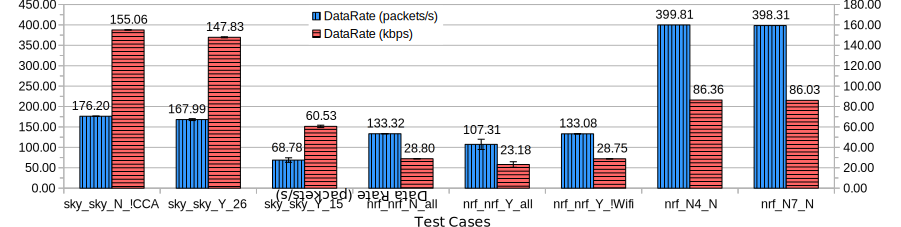
\includegraphics[width=\textwidth]{HT-dr}
\caption{Data Rate}
\label{fig:HT-dr}
\end{figure}

Note that in figure \ref{fig:HT-dr} there are two Y-axis representing the data rate in packets per second and kilobit per second. The link layer payload of 27 bytes and 110 byte was used for BLE and 802.15.4 respectively to calculate the data rate in kbps.

\begin{figure}[h]
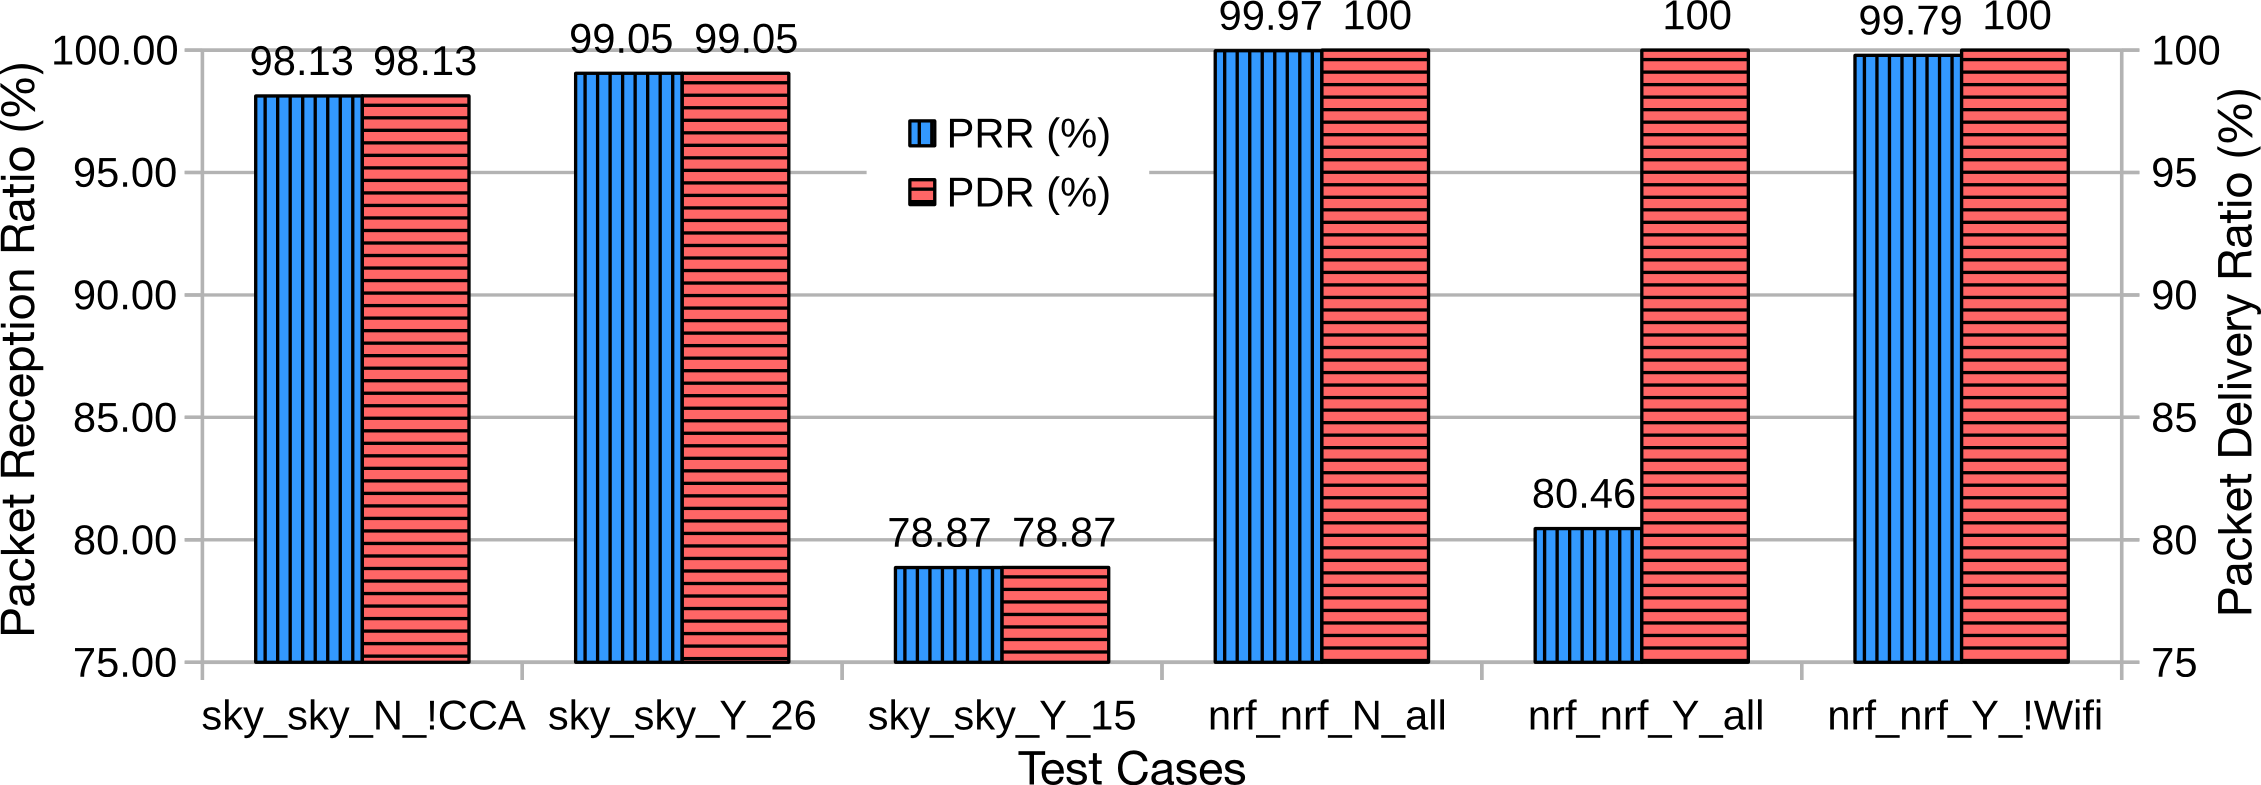
\includegraphics[width=\textwidth]{HT-r}
\caption{Reliability}
\label{fig:HT-r}
\end{figure}
The graph in figure \ref{fig:HT-r} has Y-axes from 75 to 100 \% for clearer representation of the \gls{pdr} and \gls{prr}. As mentioned in section \ref{6HTdesign} the reliability was calculate in BLE by logging the number of times the radio was switched on as this information was accessible from the SoftDevice. This allowed the calculation of \gls{prr} with one packet per connection event. Since the android devices can communicate multiple packets per connection event, the \gls{prr} could not be calculated. Hence, those test cases are not plotted.

\begin{figure}[h]
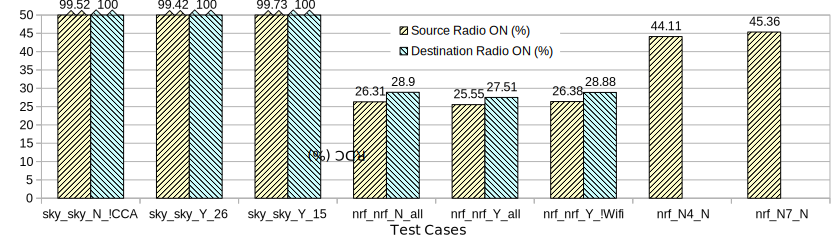
\includegraphics[width=\textwidth]{HT-ec}
\caption{Energy Consumption}
\label{fig:HT-ec}
\end{figure}

For a clearer representation of the graph, the y-axis in figure \ref{fig:HT-ec} is limited to 50\%. The break in the graph shows that when Tmote-Sky uses ~100\% of radio duty cycle.

\subsection{Analysis}
\paragraph{Data rate}
The absolute data rate is higher in 802.15.4 than BLE although the number of packets transmitter per second is higher in BLE. This is because of the higher packet size of 802.15.4, even though the bit rate of transmission of BLE is four time the bit rate of 802.15.4 at 1 Mbps.

\paragraph{Reliability}

\paragraph{Energy Consumption}

\section{\acrlong{rr} Test}


\begin{figure}[h]
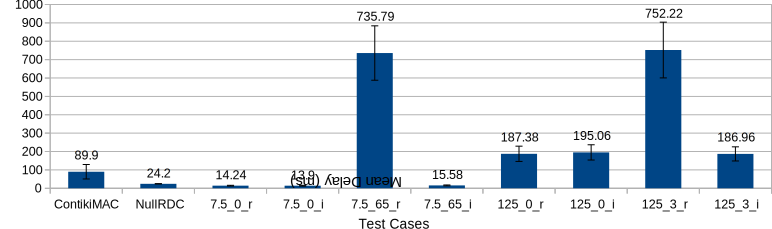
\includegraphics[width=\textwidth]{RR-l}
\caption{Latency}
\label{fig:RR-l}
\end{figure}

\begin{figure}[h]
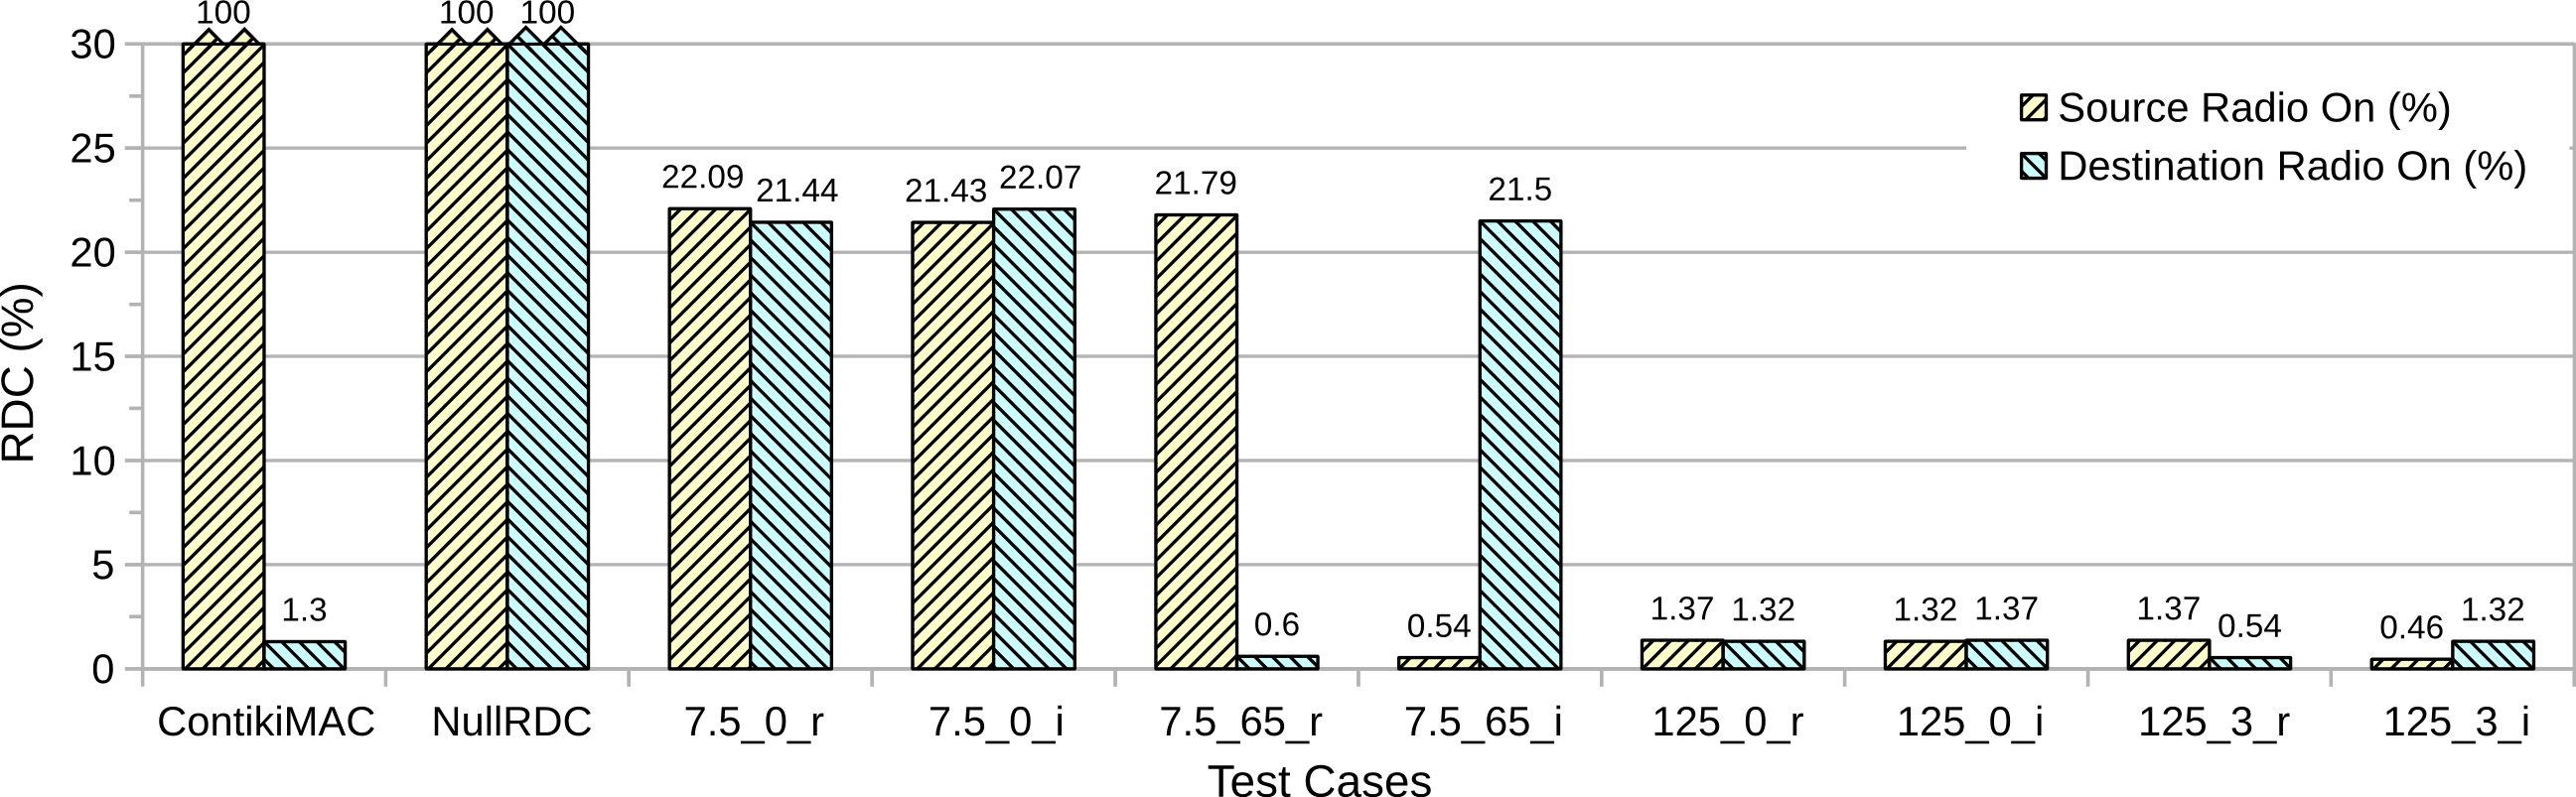
\includegraphics[width=\textwidth]{RR-ec}
\caption{Energy Consumption}
\label{fig:RR-ec}
\end{figure}

\section{What we learnt}